\chapter{Mars entry and descent}
\label{ch:entry}
Several missions have already performed entry and descent successfully  on the Martian surface. A short overview of these missions and how they descended to the surface was already given in \Cref{sec:mslref}. But for easy reference, the table with all the reference missions is given again (see \Cref{tab:mslprevmis_copy}, same as \Cref{tab:mslprevmis}).

\begin{table}[!ht]
\begin{center}
\caption{Previous Mars Entry and Descent Missions}
\label{tab:mslprevmis_copy}
\begin{tabular}{|l|l|l|l|}
\hline 
\textbf{Launch date} 		& \textbf{Country} & \textbf{Mission} & \textbf{Type} \\ \hline \hline
19 May 1971	& Soviet Union & Mars 3 & Lander (and failed rover)  \\ \hline
20 August 1975	& United States & Viking 1 & Lander \\ \hline
9 September	& United States & Viking 2 & Lander \\ \hline
4 December 1996	& United States & Mars Pathfinder/Sojourner & Lander and rover \\ \hline
2 June 2003	& Europe and United Kingdom & Mars Express/Beagle 2 & Lander \\ \hline
10 June 2003 & United States & Mars Exploration Rover - A/Spirit & Rover \\ \hline
7 July 2003	& United States & Mars Exploration Rover - B/Opportunity & Rover \\ \hline
4 August 2007 & United States & Phoenix & Lander \\ \hline
26 November 2012 & United States & Mars Science Laboratory/Curiosity & Rover \\ \hline
% 		&  &  &  \\ \hline
\end{tabular}
\end{center}
\end{table}

Also, another overview can be used to quickly show the different techniques that were used on each mission. This overview is given in \Cref{tab:overtechentdes} and is based on the information provided in \Cref{sec:mslref}.

\begin{longtable}{|l|p{4cm}|p{4cm}|p{4cm}|}
\caption{Previous entry, descent and landing methods}
\label{tab:overtechentdes}
\endfirsthead
\endhead
\hline 
\textbf{Mission} 		& \textbf{Entry phase} & \textbf{Atmospheric descent phase} & \textbf{Landing phase} \\ \hline \hline
Mars 3 		& Separated from \ac{s/c} (before entering orbit \cite{mars3_2014}, semi-direct entry), main descent engine fire to point heat shield & Heat shield, braking parachute and reefed main parachute \cite{macdonald2014} & Retro rockets (in back-shell) and drop with air-bags \cite{perminov1999} \\ \hline
Viking(s) 		& Separated from orbiter, main descent engines to de-orbit & Heat shield and parachute & Drop with retro rockets \\ \hline
Mars Pathfinder 		& Direct entry & Heat shield and parachute & Lowering cable, retro rockets (in back-shell) and air-bags  \\ \hline
Mars Express/Beagle 2 		& Separated from orbiter & Heat shield , pilot parachute and main parachute \cite{mooij2013para} & Air-bags and main parachute (still attached) \\ \hline
Mars Exploration Rover(s) 		& Direct entry & Heat shied and parachute & Lowering cable, retro rockets (in back-shell) and air-bags \\ \hline
Phoenix 		& Direct entry & Heat shield and parachute & Drop with retro rockets \\ \hline
Mars Science Laboratory 		& Direct entry & Heat shield, manoeuvres and parachute & Drop with powered descent followed by hovered descent and deployment on surface through lowering cable \\ \hline
	
% 		&  &  &  \\ \hline
\end{longtable}

The \ac{EDL} phases all show similarities between the different missions and also some distinct differences. The used methods, general theory and alternative methods will be discussed in this chapter per \ac{EDL} phase. 

%%\textcolor{red}{\textbf{Examples/illustrations of different entries?}}

In order to visualize the events described in \Cref{tab:overtechentdes}, the \ac{EDL} sequences of the Viking, \ac{MPF}, Beagle 2 and \ac{MSL} missions are given in \Cref{fig:viking1_edl_crankshaft,fig:mpf_edl_isbell1997,fig:beagle_edl_laufer2010,fig:msl_edl_brown2012} respectively. 

%
\begin{figure}[!ht]
\centering
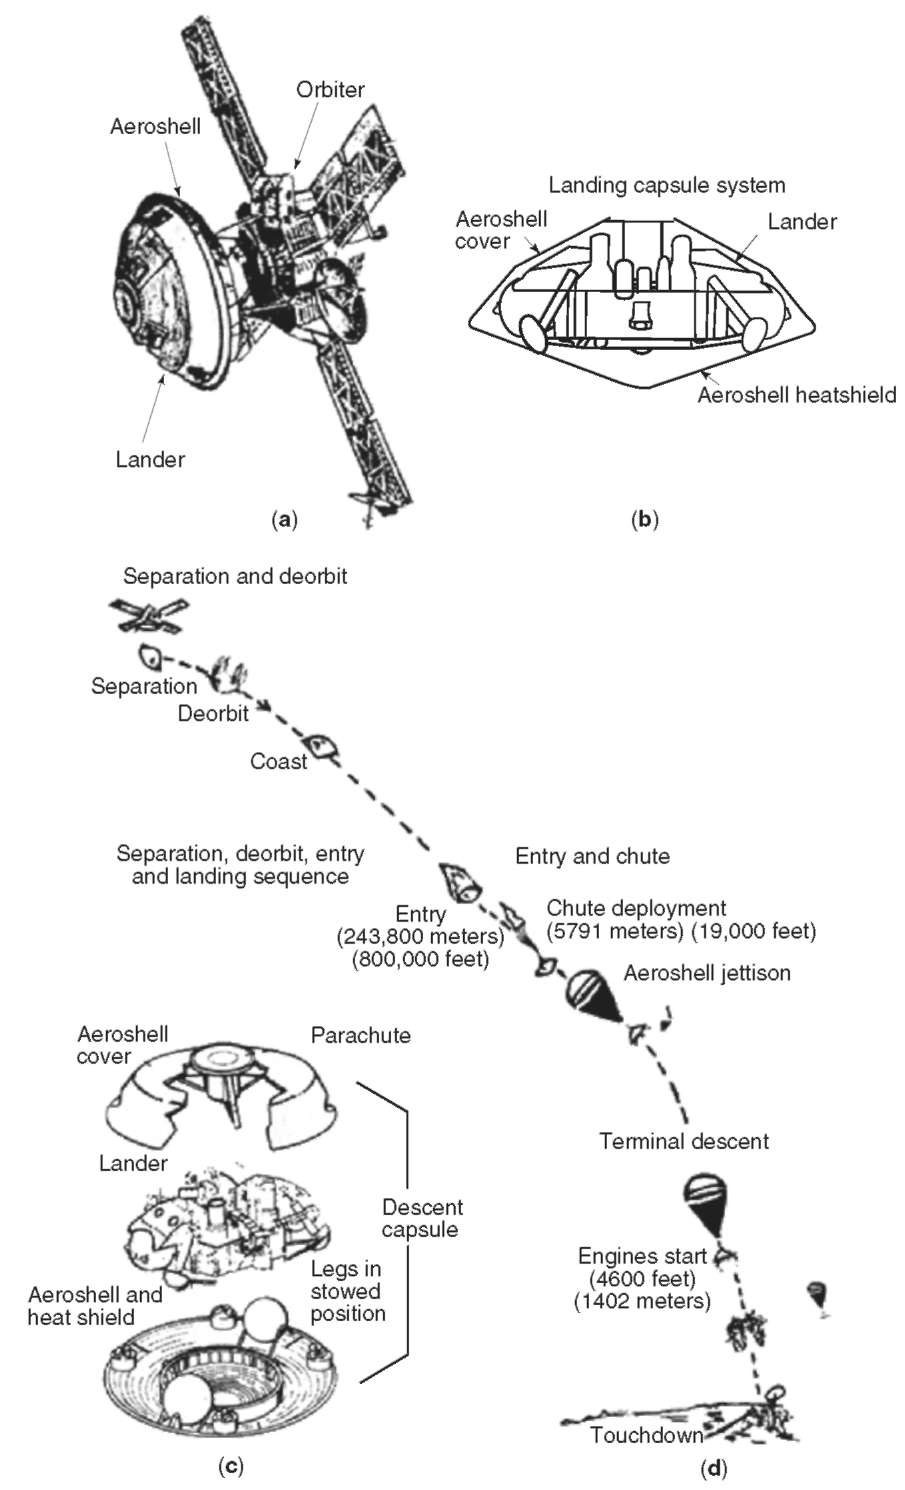
\includegraphics[width=0.5\textwidth]{figures/entry_descent/viking1_edl_crankshaft.jpg}
\caption{Illustration of the Viking 1 \cite{crankshaft}; a) the complete \ac{s/c}, b) the entry vehicle, c) exploded view and d) \ac{EDL} sequence}
\label{fig:viking1_edl_crankshaft}
\end{figure}

\begin{figure}[!ht]
\centering
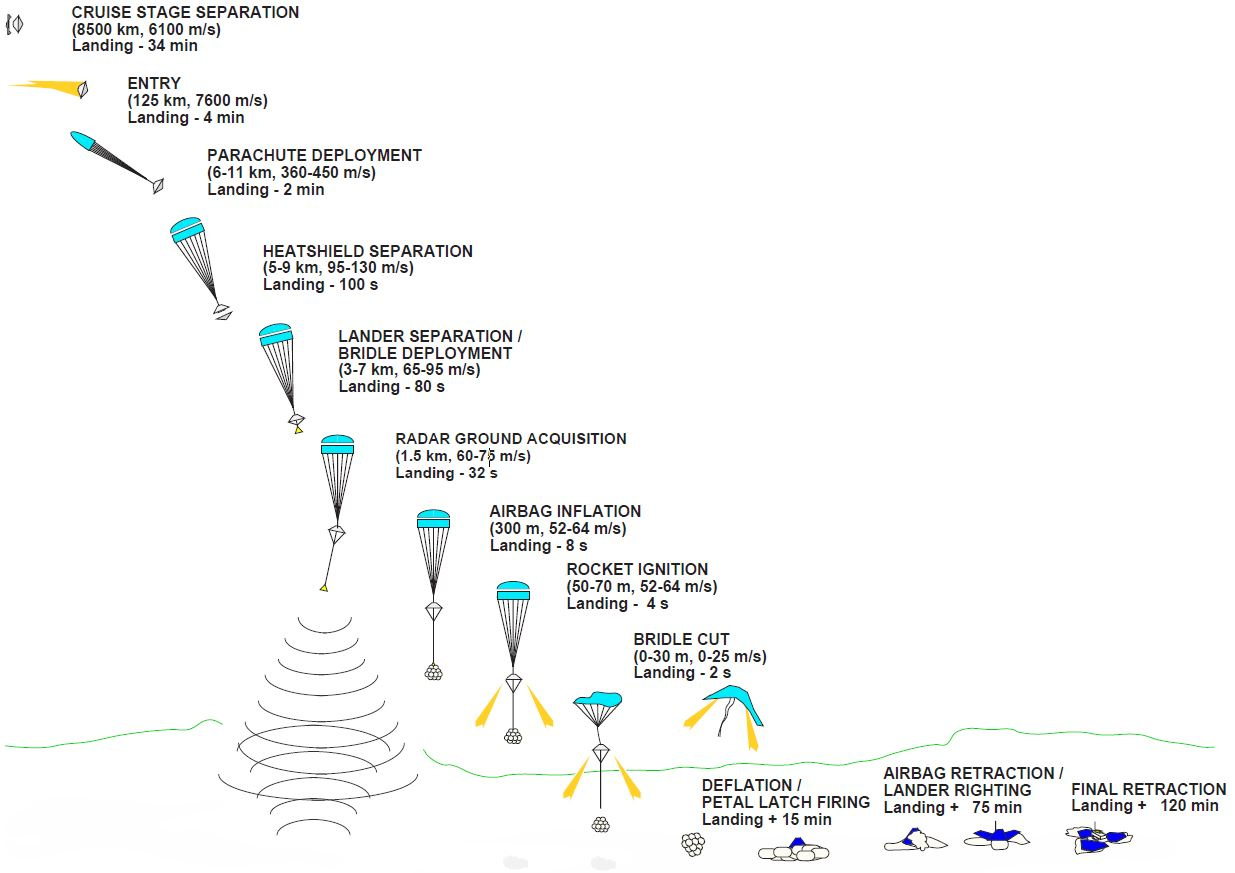
\includegraphics[width=0.7\textwidth]{figures/entry_descent/mpf_edl_isbell1997.jpg}
\caption{Illustration of the \ac{MPF} \ac{EDL} sequence \cite{isbell1997}}
\label{fig:mpf_edl_isbell1997}
\end{figure}

\begin{figure}[!ht]
\centering
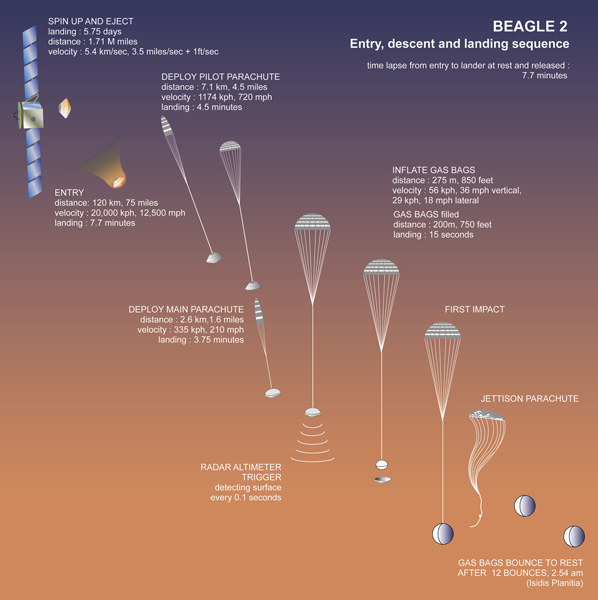
\includegraphics[width=0.7\textwidth]{figures/entry_descent/beagle_edl_laufer2010.jpg}
\caption{Illustration of the Beagle 2 \ac{EDL} sequence \cite{laufer2010}}
\label{fig:beagle_edl_laufer2010}
\end{figure}

\begin{figure}[!ht]
\centering
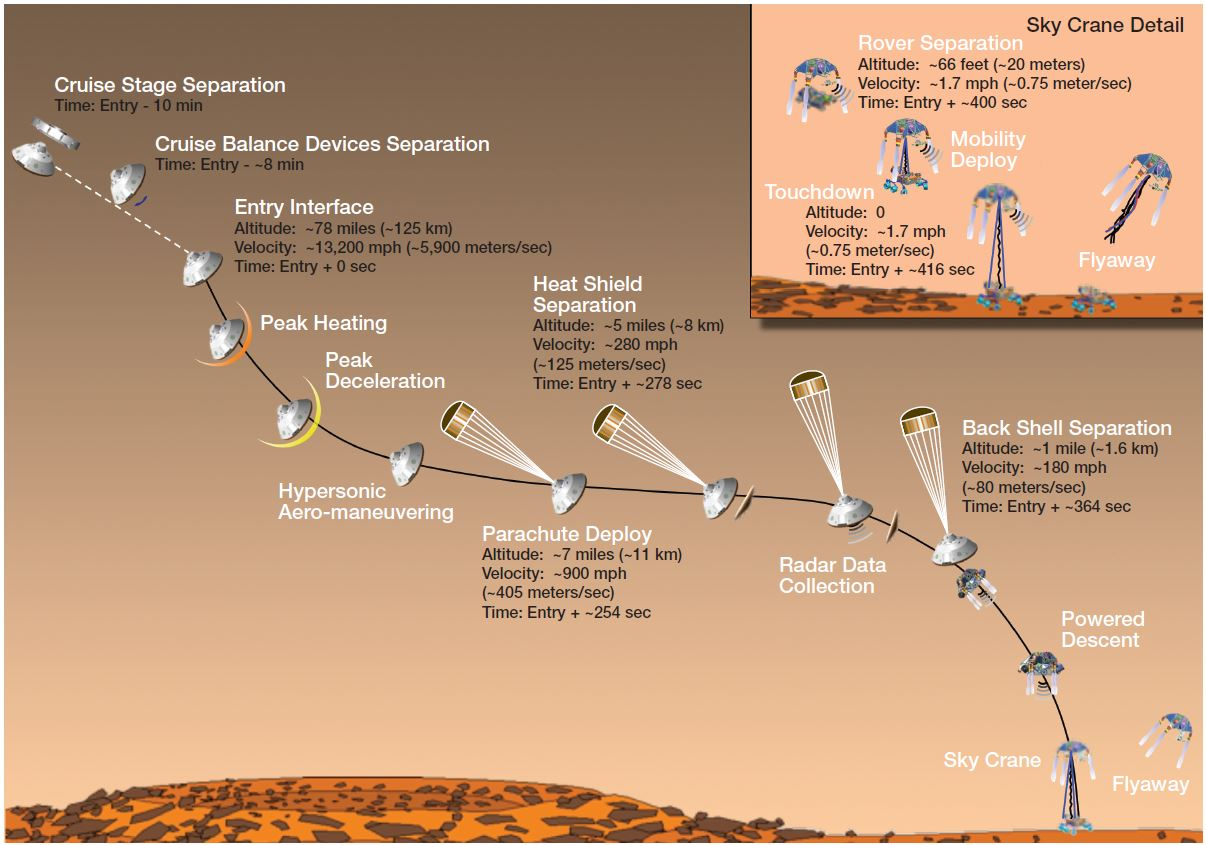
\includegraphics[width=0.7\textwidth]{figures/entry_descent/msl_edl_brown2012.jpg}
\caption{Illustration of the \ac{MSL} \ac{EDL} sequence \cite{brown2012}}
\label{fig:msl_edl_brown2012}
\end{figure}


\section{Entry phase}
\label{sec:entry}
Given the previous missions seen in \Cref{tab:overtechentdes}, it is clear that a distinction can be made between orbital entry and direct entry, with the exception of Mars 3 which performed a semi-direct entry where the entry vehicle was released before the \ac{s/c} entered orbit around Mars \cite{mars3_2014}. During the direct entry, a spacecraft intercepts Mars and enters the atmosphere with speeds higher than escape velocity (around 7.26 $km/s$ in the case of Pathfinder compared to 4.7 $km/s$ in the case of the Viking missions \cite{braun2006}, Mars escape velocity is around 5.027 $km/s$ \cite{williams2015}. When the spacecraft uses an orbital entry, the speeds are much lower, however in this case usually main engines are fired to decelerate and rotate the capsule such that the heat shield is pointed in the proper direction. The \ac{MPF}, Beagle 2 and MER missions all had no guidance and no centre of mass offset, and thus performed a purely ballistic entry \cite{mooij2013entry}. In their case, they entered the atmosphere with an angle of attack of 0$\degree$ \cite{braun2006,smith2002}. The \ac{MPF} and MER were spin stabilized at entry \cite{steltzner2006}. The Viking, Phoenix and \ac{MSL} entry vehicles all used a centre of mass offset in order to create lift and thus control the entry \cite{braun2006} (semi-ballistic \cite{mooij2013entry}). In the case of \ac{MSL}, active guidance in the form of thrusters were also used to have more control over the entry of the vehicle.   


During the entry phase the \ac{RCS}, usually thrusters, helps to assure the proper attitude of the capsule. Together with the mass and aerodynamic properties of the capsule, they make sure that the heat shield is pointed in the right direction (ballistic and semi-ballistic entry \cite{mooij2013entry}). 

\section{Atmospheric descent phase}
\label{sec:descent}
The actual atmospheric descent phase of the \ac{EDL} is in this case defined to be the phase where the atmosphere is first 'touched' by the entry vehicle. The first part of this phase is performed using a protective heat shield, and the rest of the vehicle is protected by means of an Aero-shell. More on both these aspects of the vehicle will be discussed in \Cref{subsec:heatshield}. The second part of the atmospheric descent usually consists of deceleration through the use of a parachute. Some general theory and a description of the parachutes used in the reference missions will be given in \Cref{subsec:para}. However, there are currently also alternative atmospheric decelerators that could be used instead of the traditional heat shield and parachutes. \Cref{subsec:specaerodec} provides a short overview of the different alternatives and likely candidate technologies that have already been under consideration for use in future Mars missions. 


\subsection{Aero-shell and heat-shield}
\label{subsec:heatshield}
When looking at the entry vehicle a distinction can be made between the lander (and/or rover) and the protective cover. This protective cover is called the Aero-shell and protects the lander during the cruise to Mars and during the entry and descent. It usually consists of two different segments: a heat shield in the front and a back-shell \cite{viotti2015}. A graphic representation of the aero-shell for the MER missions is given in \Cref{fig:mer_aeroshell_viotti2015}. The back-shell can house the parachute(s), extra decelerators, in this case solid rocket motors, and other subsystems such as release mechanisms for the lander.

\begin{figure}[!ht]
\centering
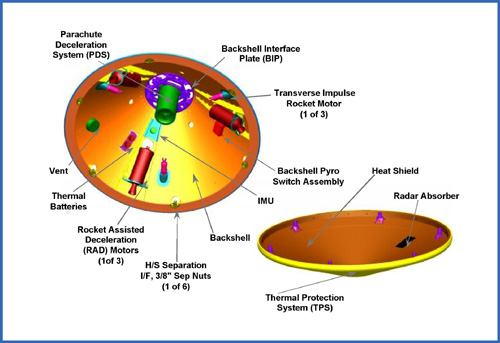
\includegraphics[width=0.7\textwidth]{figures/entry_descent/mer_aeroshell_viotti2015.jpg}
\caption{Graphic representation of the MER aero-shell \cite{viotti2015}}
\label{fig:mer_aeroshell_viotti2015}
\end{figure}

The heat shield acts both as thermal protector as well as main decelerator. Different thermal protectors exist, but in case of Mars missions, ablative thermal protection systems \acs{TPS} are used \cite{braun2006,viotti2015}. The idea behind an ablative heat shield is that energy is taken away from the vehicle by losing the shield material while it burns. Due to the hypersonic speeds ($>$ Mach 5) a bow-shock is present in front of the vehicle during entry, resulting in aerodynamic heating of the air \cite{mooij2013entry}. In \Cref{fig:marsev_mooij2013entry} a graphic representation is given of what happens when a (semi-)ballistic vehicle enters the Martian atmosphere. 

\begin{figure}[!ht]
\centering
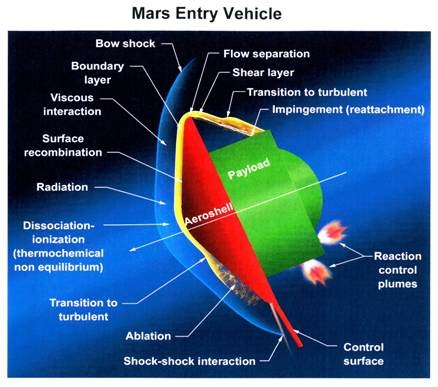
\includegraphics[width=0.7\textwidth]{figures/entry_descent/marsev_mooij2013entry.jpg}
\caption{Graphic representation of a Martian entry \cite{mooij2013entry}}
\label{fig:marsev_mooij2013entry}
\end{figure}

As can be seen in this figure, the hot air can re-attach after flow separation behind the vehicle. This is why the back-shell also requires a thermal protective layer, but not has different requirements because of the lower energy in the re-attached flow. For the design of a \acs{TPS} for a ballistic entry, three different parameters are very important: the maximum dynamic pressure ($q_{dyn,max}$), the maximum heat flux ($\dot{Q}_{max}$)(which is the energy per time per square metre) and the integrated heat flux or maximum heat load ($Q_{max}$). These maxima occur in the stagnation point on the vehicle and determine the type of \acs{TPS} material and the thickness. Another important system requirement is the maximum deceleration ($g_{load,max}$) \cite{mooij2013entry}. \Cref{fig:heatanddec_mooij2013entry} shows the general graphs for the density, vehicle velocity, deceleration and the heat flux as a function of altitude, and it is interesting to note that the peak deceleration happens at an altitude lower than the peak heat flux. More information on how to determine these maxima and how they are affected by design choices such as entry angle and entry velocity can be found in \cite{mooij2013entry}.  

\nomenclature{$q_{dyn,max}$}{Maximum dynamic pressure\nomunit{$Pa$}}
\nomenclature{$\dot{Q}_{max}$}{Maximum heat flux\nomunit{$W/m^{2}$}}
\nomenclature{$Q_{max}$}{Maximum heat load\nomunit{$J/m^{2}$}}
\nomenclature{$g_{load,max}$}{Maximum deceleration\nomunit{$m/s^{2}$}}


\begin{figure}[!ht]
\centering
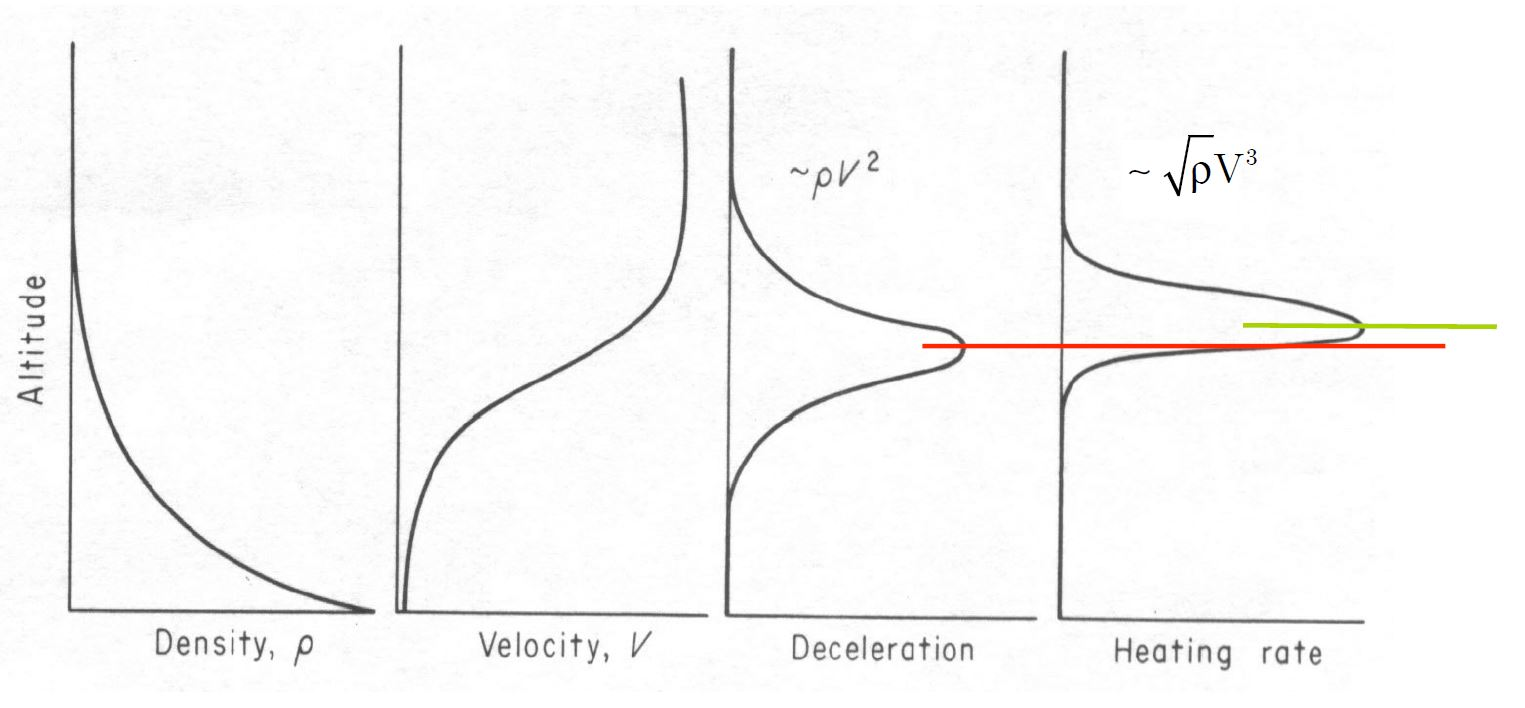
\includegraphics[width=0.7\textwidth]{figures/entry_descent/heatanddec_mooij2013entry.jpg}
\caption{Typical entry characteristic graphs \cite{mooij2013entry}}
\label{fig:heatanddec_mooij2013entry}
\end{figure}

\nomenclature{$\rho$}{Density\nomunit{$kg/m^{3}$}}
%\nomenclature{$$}{\nomunit{$$}}

The ablative material for the \acs{TPS} is therefore chosen based on the mission characteristics during entry. An overview of the ablative materials and the dimensions of the heat shields that were used in the reference missions is given in \Cref{tab:heatshieldchar} and are mostly based on \cite{braun2006} unless mentioned otherwise. Also, a comparison of the different NASA mission aero-shells is visualized in \Cref{fig:aeroshellcomp_way2007}.

\begin{table}[!ht]
\begin{center}
\caption{Previous Mars mission heat shield characteristics}
\label{tab:heatshieldchar}
\begin{tabular}{|l|l|l|l|}
\hline 
\textbf{Mission} 		& \textbf{Shield diameter [$m$]} & \textbf{\acs{TPS} material} & \textbf{\acs{TPS} thickness [$cm$]} \\ \hline \hline
Mars 3 		& 2.9 \cite{mars3_2014}& unknown & unknown \\ \hline %perminov1999
Viking(s) 		& 3.5 & \acs{SLA}-561V & 1.37 \\ \hline
Mars Pathfinder 		& 2.65 & \acs{SLA}-561V & 1.91 \\ \hline
Beagle 2 		& 0.9 \cite{smith2002}& Norcoat Liège FI 
\cite{plotard2003}& 0.8 \cite{plotard2003}\\ \hline
Mars Exploration Rover(s) 		& 2.65 & \acs{SLA}-561V & 1.57 \\ \hline
Phoenix 		& 2.65 & \acs{SLA}-561V & 1.40 \\ \hline
Mars Science Laboratory 		& 4.6 & \acs{PICA} (\acs{SLA}-561 back-shell) \cite{blau2011}& 2.29 \\ \hline


% 		&  &  &  \\ \hline
\end{tabular}
\end{center}
\end{table}

\begin{figure}[!ht]
\centering
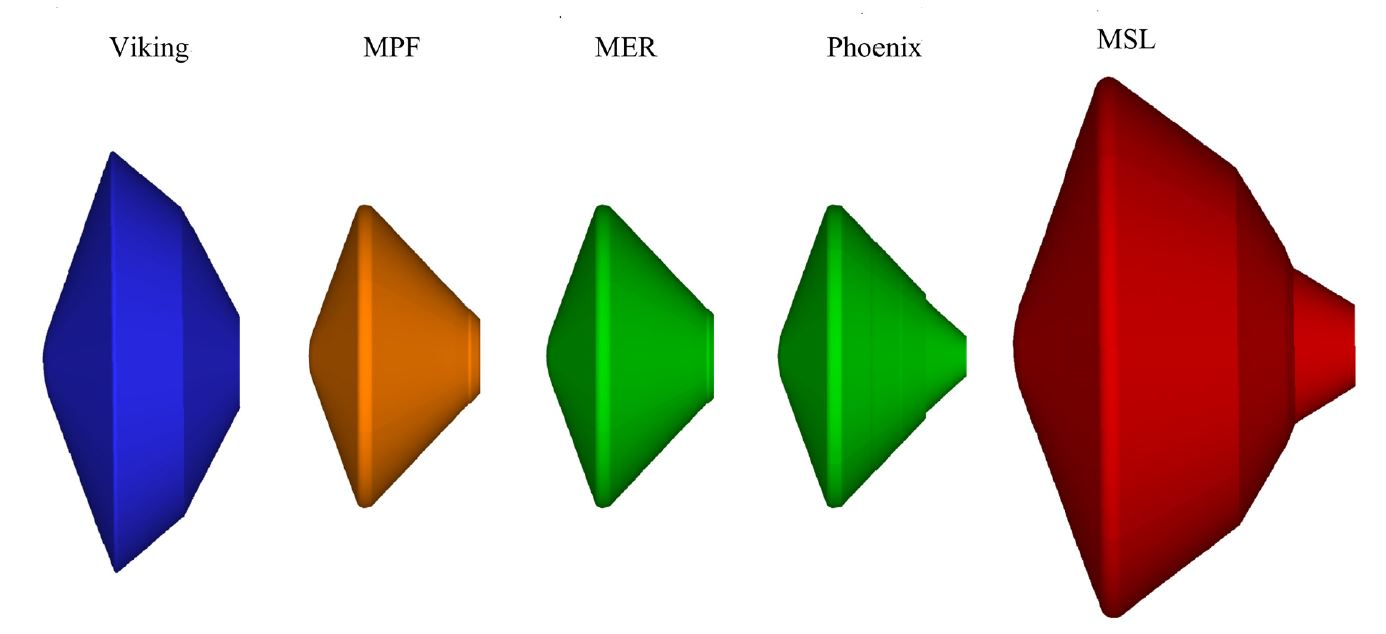
\includegraphics[width=0.7\textwidth]{figures/entry_descent/aeroshellcomp_way2007.jpg}
\caption{Aero-shell comparison of the different NASA Mars entry vehicles \cite{way2007}}
\label{fig:aeroshellcomp_way2007}
\end{figure}

The mentioned Norgot Liège \acs{TPS} used on Beagle 2 was originally developed for the Ariane 4 \cite{bouilly2006} and the French military by EADS Launch Vehicles (before called Aerospatiale, currently Airbus Defence and Space) back in the '70s \cite{plotard2003}. The Norgot Liège \acs{TPS} is produced in panels and is made from cork powder and phenolic resin. The \acs{SLA}-561V was developed by the Martin company (now Lockheed Martin) back in the '60s specifically for a mission to Mars \cite{strauss1967}. The \acf{SLA} material is a combination of elastomeric sillicone and cork \cite{martin1975} and the original \acs{SLA}-561 was used for the Space Shuttle External tank as well. And finally, the \acf{PICA} was developed by NASA in the '90s and was first successfully used for re-entry on the Stardust mission \cite{blau2011}.






\subsection{Parachutes}
\label{subsec:para}
%What determines the opening requirements of the parachute? Vehicle mass, final speed at certain altitude?
Parachutes are traditional aerodynamic decelerators that are used for atmospheric deceleration starting at supersonic or subsonic speeds ($<$ Mach 5) \cite{mooij2013para}. In 1978 the third United States Air Force Parachute Handbook was published containing information on numerous parachute designs \cite{ewing1978}. From this collection, four types of parachutes have been flown in space \cite{mooij2013para} and two were used for Mars missions: the \ac{DGB} (see \Cref{fig:dgb_mooij2013para}) and the Ringsail Parachutes (see \Cref{fig:ringsail_mooij2013para}).  

\begin{figure}[!ht]
\centering
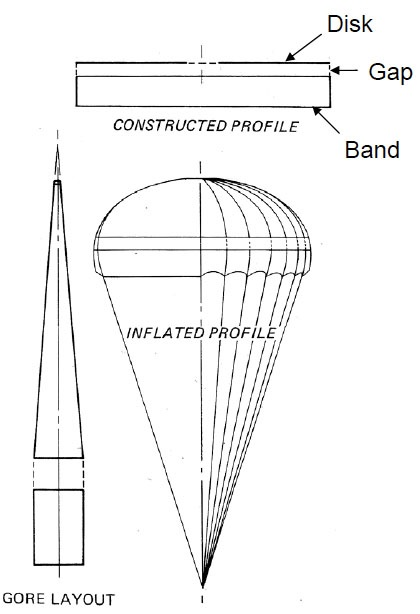
\includegraphics[width=0.4\textwidth]{figures/entry_descent/dgb_mooij2013para.jpg}
\caption{Disk-Gap Band parachute \cite{ewing1978}}
\label{fig:dgb_mooij2013para}
\end{figure}

\begin{figure}[!ht]
\centering
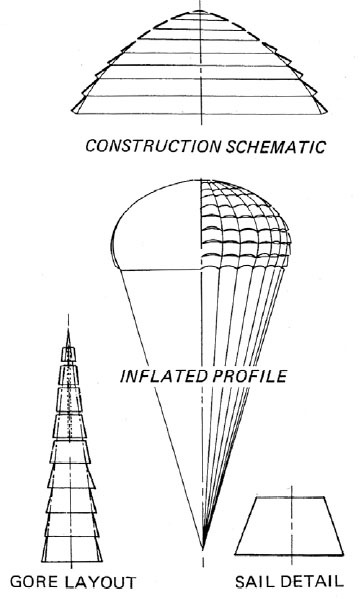
\includegraphics[width=0.3\textwidth]{figures/entry_descent/ringsail_mooij2013para.jpg}
\caption{Ringsail parachute \cite{ewing1978}}
\label{fig:ringsail_mooij2013para}
\end{figure}

The size of the parachute needed can be determined through the terminal descent conditions (or the specified conditions at a certain altitude). Assuming a circular parachute surface, the chute diameter $d_{P}$ can be determined using the expression given by \Cref{eq:chutediam}.

\begin{equation}\label{eq:chutediam}
d_{P}=2\sqrt{\dfrac{1}{\pi C_{D_{P}}}\left(2\dfrac{mg_{0,mars}}{\rho_{0}V_{f}^{2}}-C_{D_{EV}}S_{EV}\right)}
\end{equation}

\nomenclature{$d_{P}$}{Parachute diameter\nomunit{$m$}}
\nomenclature{$C_{D_{P}}$}{Parachute drag coefficient\nomunit{$-$}}
\nomenclature{$m$}{System mass\nomunit{$kg$}}
\nomenclature{$g_{0,mars}$}{Gravitational acceleration at the Martian surface\nomunit{$m/s^{2}$}}
\nomenclature{$\rho_{0}$}{Air density at the Martian surface\nomunit{$kg/m^{3}$}}
\nomenclature{$V_{f}$}{Desired final velocity\nomunit{$m/s$}}
\nomenclature{$S_{EV}$}{Surface area of the entry vehicle\nomunit{$m^{2}$}}
\nomenclature{$C_{D_{EV}}$}{Drag coefficient of the entry vehicle\nomunit{$-$}}
\nomenclature{$\beta$}{Balistic coefficient\nomunit{$kg/m^{2}$}}
%\nomenclature{$$}{\nomunit{$$}}

Here, $C_{D_{P}}$ is the drag coefficient of the parachute determined by the parachute type and given in \cite{ewing1978}, $m$ is the mass of the entire system (so both entry vehicle and parachute system), $g_{0,mars}$ is the gravitational acceleration at the Martian surface, $\rho_{0}$ is the air density at the Martian surface, $V_{f}$ is the desired final velocity, $S_{EV}$ is the surface area of the entry vehicle and $C_{D_{EV}}$ is the drag coefficient of the entry vehicle. These last two parameters can be combined with the mass $m$ to give the ballistic coefficient $\beta=\dfrac{m}{C_{D_{EV}}S_{EV}}$, which is a characteristic parameter of the entry vehicle. In that case the equation for the chute diameter can be written as given by \Cref{eq:chutediambeta}.

\begin{equation}\label{eq:chutediambeta}
d_{P}=2\sqrt{\dfrac{1}{\pi C_{D_{P}}}\left(2\dfrac{m^{2}g_{0,mars}}{\rho_{0}V_{f}^{2}}-\beta\right)}
\end{equation}

As a reference, the characteristic parameters and type of parachute(s) used in the given reference missions are shown in \Cref{tab:refparachar}. The data in the table was obtained from \cite{braun2006,cruz2006} unless mentioned otherwise. Also, given the lack of information on the Mars 3 mission, this mission will not be used as reference here.

\begin{table}[!ht]
\begin{center}
\caption{Previous Mars Mission parachute and entry vehicle characteristics}
\label{tab:refparachar}
\begin{tabular}{|l|p{3cm}|p{2cm}|p{3cm}|p{3cm}|}
%\begin{longtable}{|l|p{3cm}|p{2cm}|p{3cm}|p{3cm}|}
%\caption{Previous Mars Mission parachute and entry vehicle characteristics}
%\label{tab:refparachar}
%\endfirsthead
%\endhead
\hline 
\textbf{Mission} 		& \textbf{Parachute type} & $\mathbf{d_{P}}$ $\mathbf{[m]}$ & $\mathbf{C_{D_{P}}}$ $\mathbf{[-]}$ & $\mathbf{\beta}$ $\mathbf{[kg/m^{2}]}$  \\ \hline \hline
Viking(s) 		& \ac{DGB} & 16.2 & 0.67 & 64\\ \hline
Mars Pathfinder & \ac{DGB} & 12.7 & 0.4 & 63\\ \hline
Beagle 2 		& \ac{DGB} (Pilot), Ringsail (Main) & 3.2 (Pilot), 10.0 (Main) & 0.52 to 0.58 \cite{ewing1978}(Pilot), 0.92 \cite{fallon2005} (Main) & 73 \cite{lafleur2011}\\ \hline
Mars Exploration Rover(s) 		& \ac{DGB} & 14.1 & 0.48 & 94\\ \hline
Phoenix 	& \ac{DGB} & 11.7 & 0.67 & 65 \cite{lafleur2011}\\ \hline
Mars Science Laboratory 	& \ac{DGB} & 19.7 & 0.67 & 140 \cite{lafleur2011}\\ \hline
	
% 		&  &  & & \\ \hline
%\end{longtable}
\end{tabular}
\end{center}
\end{table}

In case of the Beagle 2, a \ac{DGB} pilot chute was used for the initial deceleration and stabilization after the heat shield deceleration and it was also used to deploy the main parachute. Also, please note that the ballistic coefficients mentioned are those at atmospheric entry. 

\subsection{Special aerodynamic decelerators}
\label{subsec:specaerodec}
The parachutes have thus far worked because the vehicle mass and speeds were low enough, however when the masses and speeds become higher for say a manned mission to Mars, the traditional aerodynamic decelerators will simply not be sufficient to make a soft landing on the Martian surface \cite{nasafacts2013}. Also, because of the surface elevation, it is currently impossible to reach approximately half of the surface with the currently used techniques. Fortunately other high speed (far into the hypersonic regime) alternatives have been envisioned and tested in as early as the '50s. These alternative decelerators can be divided up into three categories: hypersconic parachutes (made out of fabric and have a close resemblance to traditional parachutes) \cite{lingard2005}, trailing inflatable aerodynamic decelerators \acs{IAD} (are parachute like inflatable devices) and attached \acs{IAD}s (have a close resemblance to      inflatable heat shields but are not always used for the initial deceleration from high hypersonic speeds; around Mach 30).

Two examples of hypersonic parachutes are the hyperflo and the supersonic-x parachutes. The hyperflo parachute was developed in the '60s and is described by \cite{pepper1968}. It is a flat circular ribbon weaved parachute capable of resisting aerodynamic heating and can be deployed at speeds up to at least Mach 6 \cite{lingard2005}. A photo and graphic representation of the chute if given in \Cref{fig:hyperflo_lingard2005}.

\begin{figure}[!ht]
\centering
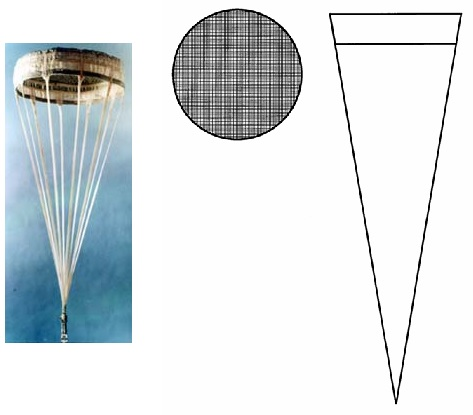
\includegraphics[width=0.4\textwidth]{figures/entry_descent/hyperflo_lingard2005.jpg}
\caption{Hyperflo parachute \cite{lingard2005}}
\label{fig:hyperflo_lingard2005}
\end{figure}   

The other hypersonic parachute, the supersonic-x, was also developed in the '60s \cite{galigher1969}, and has been tested up to Mach 8 \cite{ewing1978}. Its main use would be as a drogue parachute because of the parachute stability but only average drag. It has a close resemblance to a reversed bell nozzle as can be seen in \Cref{fig:supersonicx_ewing1978}. 

\begin{figure}[!ht]
\centering
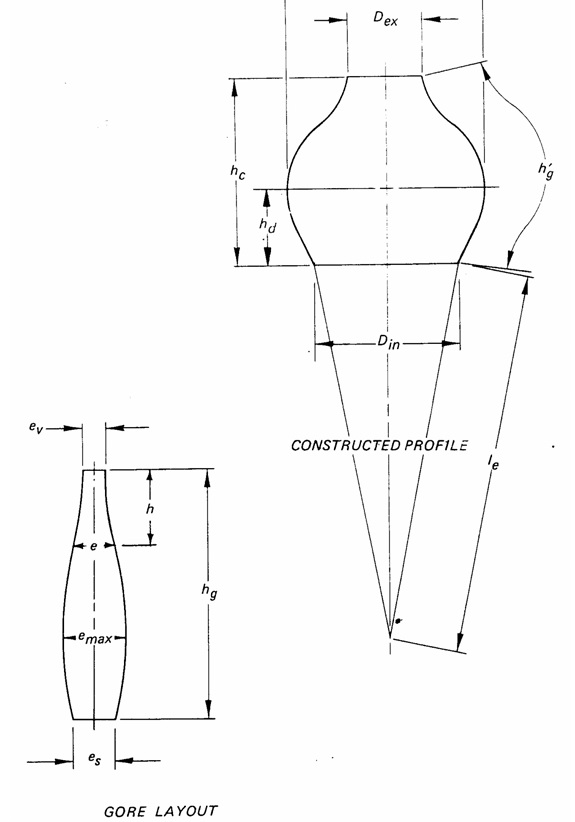
\includegraphics[width=0.4\textwidth]{figures/entry_descent/supersonicx_ewing1978.jpg}
\caption{Supersonic-x parachute \cite{ewing1978}}
\label{fig:supersonicx_ewing1978}
\end{figure}  

Both of these designs were rigorously tested in the '60s but seem not to have any merit in current investigations into Martian decelerators. \acs{IAD}s on the other hand seem to have gained much popularity in the past few years (see for instance \cite{mooij2013para,gallon2013,sostaric2010,nasafacts2013,clark2009,steinfeldt2006,witkowski2006}). 
The earliest trailing \acs{IAD} developed was the so called ballute (a balloon parachute) by Goodyear in the '50s and was part of the Gemini escape system \cite{mooij2013para}. A photo of the original design is shown in \Cref{fig:ballute_mooij2013para}. Currently, the design is under consideration to perform as a drogue chute for hypersonic Mars entries combined with an improved supersonic ringsail main parachute and an attached \acs{IAD} \cite{gallon2013}. 

\begin{figure}[!ht]
\centering
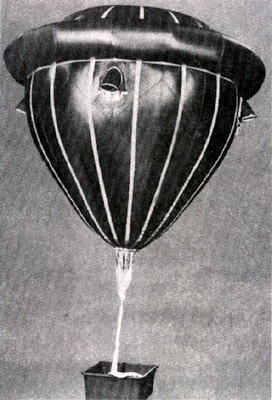
\includegraphics[width=0.2\textwidth]{figures/entry_descent/ballute_mooij2013para.jpg}
\caption{The original ballute by Goodyear \cite{mooij2013para}}
\label{fig:ballute_mooij2013para}
\end{figure} 

Other examples of trailing \acs{IAD}s currently under consideration are shown in \Cref{fig:trailingiad_mooij2013para}.

\begin{figure}[!ht]
\centering
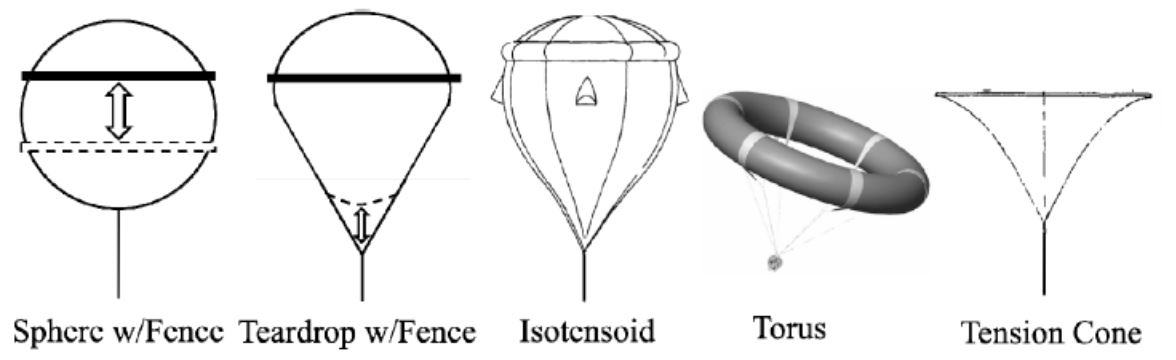
\includegraphics[width=0.6\textwidth]{figures/entry_descent/trailingiad_mooij2013para.jpg}
\caption{Selection of trailing \acs{IAD}s under investigation \cite{mooij2013para,witkowski2006}}
\label{fig:trailingiad_mooij2013para}
\end{figure} 

One of the earliest examples of an attached \acs{IAD} was developed in the '60s as well \cite{deveikis1970} and underwent several supersonic tests. A graphic representation of such a decelerator is given in \Cref{fig:attachediad_deveikis1970}. 

\begin{figure}[!ht]
\centering
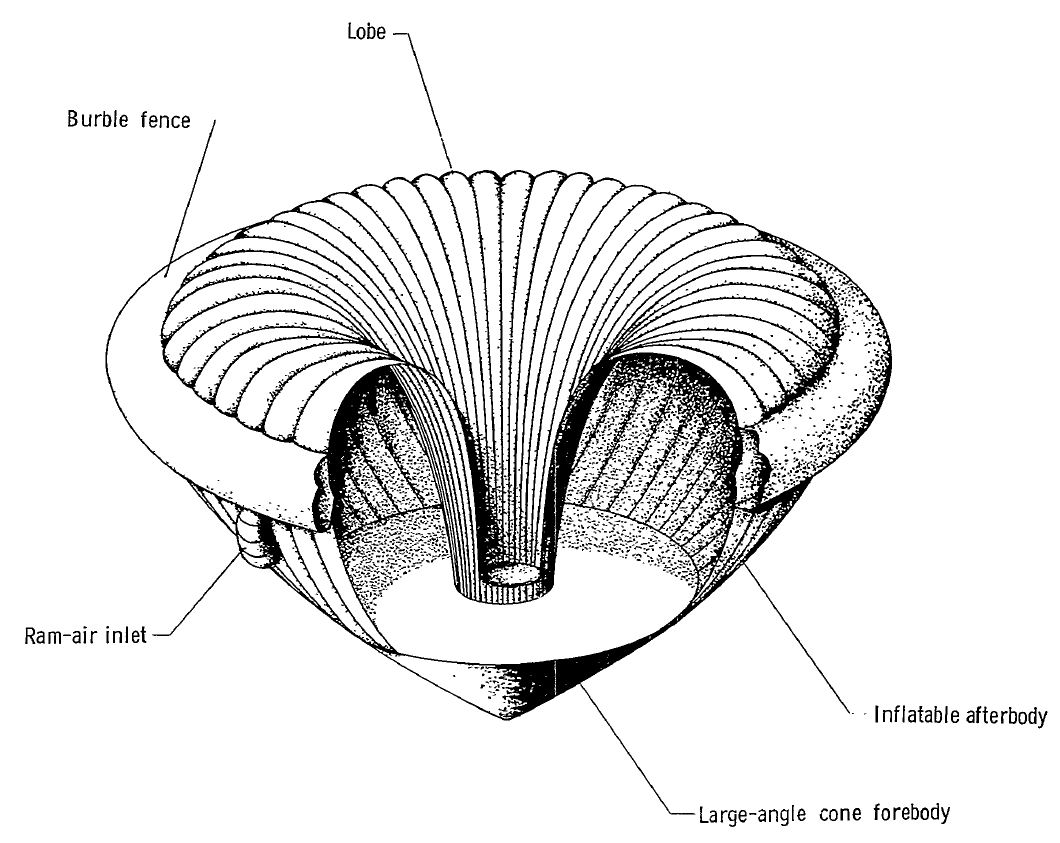
\includegraphics[width=0.5\textwidth]{figures/entry_descent/attachediad_deveikis1970.jpg}
\caption{Earliest design of an attached \acs{IAD} \cite{deveikis1970}}
\label{fig:attachediad_deveikis1970}
\end{figure}

Another supersonic attached \acs{IAD} is the tension cone \cite{clark2009,steinfeldt2006} (see \Cref{fig:attachediad_mooij2013para} for examples of attached \acs{IAD}s). This supersonic \acs{IAD} could be used in combination with a hypersonic heat shield \acs{IAD} (stacked toroid blunted cone in the figure) to perform a Martian re-entry \cite{sostaric2010}. 

\begin{figure}[!ht]
\centering
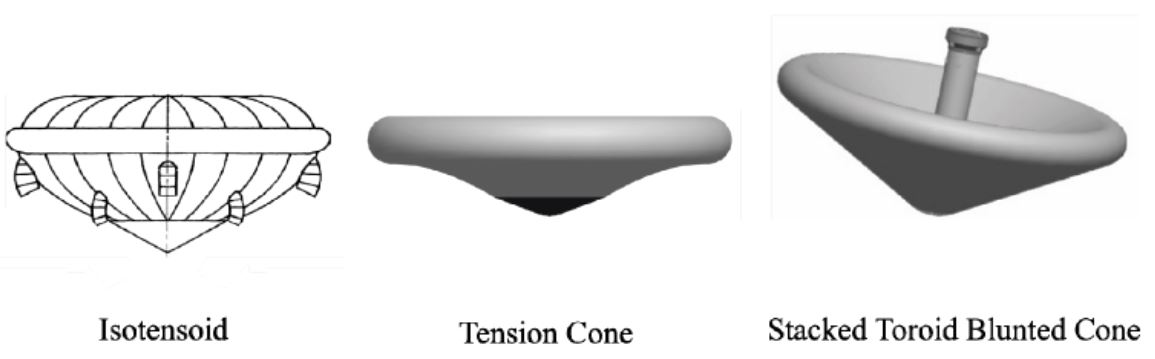
\includegraphics[width=0.6\textwidth]{figures/entry_descent/attachediad_mooij2013para.jpg}
\caption{Different attached \acs{IAD}s\cite{mooij2013para}}
\label{fig:attachediad_mooij2013para}
\end{figure}

Considering all the different possible alternatives for aerodynamic decelerators it is clear that there are currently plenty of options under development, but it is unclear at the moment which (combination) of these will perform best in case of for instance the \ac{MSL} 2 mission. 


\section{Landing phase}
\label{sec:landing}
The landing is defined as the final approach to the surface. In this phase, the final velocity is brought down to the required touchdown speed using the final deceleration systems. In this phase, there are several methods of getting the lander/rover safely on the planet surface. These methods were already mentioned in \Cref{tab:overtechentdes}, and usually involved a combination of the different methods. In this section, the methods are divided up into the use of retro rockets, lowering cable(s) and air-bags. A clearer overview of the different methods used per reference mission is shown in \Cref{tab:landingref}.

\begin{table}[!ht]
\begin{center}
\caption{Landing methods used by previous Mars missions}
\label{tab:landingref}
\begin{tabular}{|l|c|c|c|}
\hline 
\textbf{Mission}  		& \multicolumn{3}{c|}{\textbf{Method used}} \\ \cline{2-4}
& \textbf{Retro rockets} & \textbf{Lowering cable(s)} & \textbf{Air-bags}  \\ \hline \hline
Mars 3 		& Yes (in back-shell) & No  & Yes \\ \hline
Viking(s) 		& Yes & No & No \\ \hline
Mars Pathfinder 		& Yes (in back-shell) & Yes & Yes \\ \hline
Beagle 2 		& No & No & Yes \\ \hline
Mars Exploration Rover(s) 		& Yes (in back-shell) & Yes & Yes \\ \hline
Phoenix 		& Yes & No & No \\ \hline
Mars Science Laboratory 		& Yes (in hover-crane) & Yes & No \\ \hline
 		
% 		&  &  &  \\ \hline
\end{tabular}
\end{center}
\end{table}
 
In the next subsections, the use of the different methods will be discussed in case of the different reference missions.

\subsection{Retro rockets}
\label{subsec:retrock}
Retro rockets were used in almost all of the reference missions. The reason to use them is to provide high final deceleration and controlled descent \cite{mooij2013para}. The Mars 3 lander used gunpowder engines to perform a final deceleration before the lander was dropped \cite{perminov1999}. Both the \ac{MPF} and the MER missions used solid retro rockets to decelerate during final approach \cite{pathfinder_jpl1997,bonnefond2006}.
On the Viking, and \ac{MSL} missions the retro rockets were liquid monopropellant engines that could be throttled for better control of the precise landing \cite{way2007,soffen1977}. The Phoenix engines were also liquid monopropellant engines, but instead it was decided to go for a pulse mode modulated system \cite{mcallister2009}.

\subsection{Lowering cable}
\label{subsec:lowcab}
In three cases, lowering cables (or bridles) were used during the final approach phase. For the \ac{MPF} and MER missions the lowering cable acted as a tether and provided space for the air-bags to deploy, a safe distance from the solid retro rockets and increased stability \cite{pathfinder_jpl1997}.
In case of the \ac{MSL}, the lowering cables were used slightly differently. \ac{MSL} had three of them, and they were used for controlled descent unto the Martian surface rather than a tether \cite{way2007}. Only when it was confirmed that the rover had landed on the surface (cables would have less tension on them), the cables were cut and moved away with the hovering crane. The lowering of the rover on the surface via cables was preferred because this would minimize soil contamination and provide less risk to the rover itself. 

\subsection{Air-bags}
\label{subsec:airbags}
And finally, four missions (the smaller landers/rovers) used air-bags to dampen the impact on the Martian surface. This does not guarantee a precise landing but does provide protection for the on-board electronics and is simpler and has a lower mass compared to a powered descent unto the surface. However, when looking at future missions with higher mass requirements, air-bags might not be a viable option anymore \cite{mppg2012}.

